% !TeX root = ../main.tex
\clearpage
\section*{附录5\quad 补充对照实验与核验记录}
\phantomsection\label{appendix:experiments-r8p}
\addcontentsline{toc}{section}{附录5：补充对照实验与核验记录}

本附录整理已保存的六组专项证据，本轮仅核对身份、汇总量和文字适用范围，不重新求解。原三城主案例、原算法章节的消融与压力测试仍留在原位置。各组输入、设备、窗口和费用口径独立；公开计量、公开天气驱动的设计原型与合成数学场景分别标注，不能将其改善率相加或视为同一工程收益。以下E编号沿用随附证据索引；精确路径、SHA-256及本轮只读核对见\path{review/experiment_evidence_r8p.json}。

\begin{longtable}{@{}L{0.13\linewidth}L{0.29\linewidth}L{0.50\linewidth}@{}}
\caption{补充验证的对象、分母与已有结果}\label{tab:minor-evidence}\\
\toprule
证据与模块 & 冻结对象与比较条件 & 结果及限制\\\midrule
\endfirsthead
\toprule
证据与模块 & 冻结对象与比较条件 & 结果及限制\\\midrule
\endhead
\bottomrule
\endfoot
E01\newline 代表日权重 & 六栋BDG2海外计量建筑，同8--10个实际代表日，五类输出共30条记录 & 软/硬归一$W_1$中位数12.3150\%/4.4775\%；六例硬LP成功，统计准入3/6增至4/6，两例原峰丢失拒绝。仅验证完整日统计压缩。\\
E02\newline 厂家曲线 & 三城、两型号固定单模块，同资产、同服务2880小时，六组调度/恒温对照 & 电量费下降1.1013\%--1.5970\%，用电均增加；厂家工况与理想部分负荷假设下的有限LP，不含采购投资或当地实账。\\
E03\newline 建筑热惯性 & 双楼连续2880小时，纯热容倍率和公用电上限四格 & 增大热容省费但增加电量与固定因子碳排；公用上限使热容省费少150.52元。四格gap为0，独立守恒与状态核验通过。\\
E04\newline 管网反馈 & 72小时参考管网，无/有设计惩罚各三轮，交付191.5475~kWh相同 & 每组保留两轮不合格模式，第三轮压降237.96~Pa/m、远端供水57.45~$^\circ$C，满足300~Pa/m、55~$^\circ$C；无惩罚电量费178.64增至224.26元。有限稳态星型设计网络。\\
E08\newline 四楼连续 & 武汉合成参数数学场景，固定规划投资；8784小时服务年与2928小时声明冬季 & 两组逐楼状态/舒适/初末检查均零违约；运行gap为0.1344\%和0.4755\%。不能证明投资层或真实现场性能。\\
E09\newline 策略选取 & 已见三城，各九条固定策略，六权重、四预算；27条连续轨迹、72条选择 & 频数/软校准实际合格9/12、11/12；四种硬方法均12/12且库内遗憾为0。新候选没有胜过硬$W_1$的选策证据，费用与能量估计排序不同。\\
\end{longtable}

\subsection*{5.1\quad E01：六栋真实计量负荷的完整分母}
2017年热水、蒸汽、冷水各两栋，均未用于原开发建筑集合；站点均已见，故不声称未见站点泛化。先按计量及联合温度覆盖率至少95\%、非负有效记录等规则筛选，再冻结六栋，求解或统计门槛失败后不换样本。来源准入共记录66次判断，接受6次、拒绝60次，理由随选取记录保存。已有九例只作开发参考，不并入本六例的分母。基础聚类$K=6$、种子42，加极端锚点后实际代表日为8--10个；三种候选均使用同一组真实日，不填缺失小时、不改测值。

归一误差为$W_1/\overline L$，$\overline L$采用保留完整日的平均负荷。硬候选采用成熟线性规划，在日数守恒、完整日能量等式、极端日权重至少1日及普通日至少$10^{-6}$日条件下最小化一维CDF积分误差；软候选仍用原正则化$10^{-4}$，不能称能量硬保证。采用规则为预登记研究门槛：相对能量误差不超过0.1\%、$W_1$不劣于未校准极端日、保留范围峰值/最大爬坡及原有效观测峰全部保留。它不是官方工程验收要求。

\begin{table}[H]
\centering
\caption{六栋建筑全部权重候选及采用结果，$W_1$列单位为\%}\label{tab:r8p-bdg2-all}
\begin{tabularx}{\linewidth}{@{}Yrrrrcc@{}}
\toprule
建筑短名/类别 & 日数 & 代表日 & 频数 & 软 & 硬 & 软/硬采用\\\midrule
Alissa/热水 & 320 & 8 & 22.0936 & 18.0043 & 4.8097 & 是/是\\
Ian/热水 & 345 & 10 & 16.0723 & 10.0363 & 4.9463 & 否/否\\
Brandon/蒸汽 & 304 & 9 & 17.6675 & 20.9090 & 4.1453 & 否/是\\
Genoveva/蒸汽 & 276 & 9 & 8.2654 & 8.2519 & 3.8920 & 是/是\\
Angela/冷水 & 338 & 9 & 14.8176 & 14.5937 & 5.4304 & 否/否\\
Dorethea/冷水 & 338 & 9 & 2.9310 & 2.7885 & 2.0065 & 是/是\\\midrule
全六例中位数 & -- & -- & 15.4450 & 12.3150 & 4.4775 & 3/6、4/6\\
\bottomrule
\end{tabularx}
\end{table}

短名对应完整ID：Alissa为\path{Bobcat_education_Alissa}，Ian为\path{Eagle_assembly_Ian}，Brandon为\path{Bull_assembly_Brandon}，Genoveva为\path{Cockatoo_assembly_Genoveva}，Angela为\path{Bobcat_education_Angela}，Dorethea为\path{Bull_assembly_Dorethea}。六例硬LP均成功，最大绝对相对能量残差$3.58\times10^{-15}$，这是保留范围内的数值守恒。Brandon软校准虽然改善能量偏差，却使$W_1$比频数更差而被拒绝；硬方法没有该劣化。

\begin{table}[H]
\centering
\caption{完整日筛选损失与原观测峰诊断（全部六例）}
\begin{tabularx}{\linewidth}{@{}Yrrrr@{}}
\toprule
短名 & 有效小时 & 排除有效小时 & 排除观测能量/\% & 原峰保留/\%\\\midrule
Alissa & 8641 & 961 & 34.7855 & 100.0000\\
Ian & 8638 & 358 & 11.0041 & 97.9006\\
Brandon & 8566 & 1270 & 25.7411 & 100.0000\\
Genoveva & 8647 & 2023 & 29.6328 & 100.0000\\
Angela & 8721 & 609 & 11.4317 & 99.9682\\
Dorethea & 8742 & 630 & 4.5866 & 100.0000\\
\bottomrule
\end{tabularx}
\end{table}

两例硬候选的拒绝原因均为原观测峰保留失败，而非LP不可行；频数回退也未通过研究门槛。排除能量的分母是所有有效计量小时的已观测能量，不是填补后的全年能量。仅在完整日比较的峰值为100\%时，仍可能漏掉原观测峰，故必须保留此第二张表。历史\path{selected_method}有四条硬候选错标为软方法，已有只改标签的勘误旁表；本轮按\path{candidate_method}和\path{statistical_candidate_adopted}读取，原结果和锁不改。

\noindent\textbf{记录入口：}\path{docs/implementation_20261002/algorithm_hard_weights/}，含\path{protocol.json}、\path{selection.json}（含来源准入拒绝）、\path{results.json}、\path{adoption_records.json}、\path{failures.json}、\path{run_manifest.json}、\path{independent_verification.json}与\path{method_identity_erratum.json}。30条方法记录和六个LP见证已有独立CDF重建检查；没有成本、投资、舒适度、储热或完整时序调度认证。

\subsection*{5.2\quad E02：三城两型号厂家工况与固定资产调度}
TICA TCAV035BHE、TCAV065BHE分别取同型号有效制热量$Q$/输入功率$P$后求COP，不跨型号拼接；两型号合计165对$Q/P$数据，分别83、82对，空白工况保持缺失。单整模块数量固定，出水45~$^\circ$C，90~kW电阻备用及100~kW接电上限；理想小时占空比例不代表厂家实测变频、除霜或启停性能。研究规模为20个相同48~m$^2$公共原型的合成缩放，不是20栋现场建筑。

每城同一2880小时天气、20--27~$^\circ$C与初末20~$^\circ$C，恒温基准与全窗完美预知LP同资产、同服务。湖北条件分时电价及0.4044~kg/kWh平均因子共同用于三城，以隔离方法与天气；不是乌鲁木齐、固原当地电费或边际碳排，武汉账户资格也未核验。

\begin{table}[H]
\centering
\caption{六组厂家曲线对照全量结果；变化量为优化减恒温基准}
\begin{tabularx}{\linewidth}{@{}Yrrrr@{}}
\toprule
城市/型号后缀 & 基准电量费/元 & 优化电量费/元 & 节费/\% & 电量变化/kWh\\\midrule
乌鲁木齐/035 & 60174.37 & 59375.62 & 1.3274 & +1398.80\\
乌鲁木齐/065 & 42787.78 & 42313.34 & 1.1088 & +753.51\\
固原/035 & 62513.27 & 61605.21 & 1.4526 & +1548.64\\
固原/065 & 44657.69 & 44165.89 & 1.1013 & +874.83\\
武汉/035 & 15384.19 & 15210.85 & 1.1268 & +364.93\\
武汉/065 & 14889.78 & 14651.99 & 1.5970 & +728.99\\
\bottomrule
\end{tabularx}
\end{table}

\begin{table}[H]
\centering
\caption{六组优化用电与相对基准的参考碳排增量}
\begin{tabularx}{\linewidth}{@{}Ycrr@{}}
\toprule
城市 & 型号 & 优化电量/kWh & 碳排增量/kg\\\midrule
乌鲁木齐 & 035 & 79659.35 & 565.67\\
乌鲁木齐 & 065 & 56422.54 & 304.72\\
固原 & 035 & 83685.01 & 626.27\\
固原 & 065 & 59748.50 & 353.78\\
武汉 & 035 & 20948.64 & 147.58\\
武汉 & 065 & 20493.54 & 294.80\\
\bottomrule
\end{tabularx}
\end{table}

六组状态、服务及数值对偶检查均通过；严格下界另按有限binary64电量费LP的有理数弱对偶构造，只限定本次目标。历史比较表的对偶列仍是数值估计，不把它改称严格下界，更不推导碳排或资本支出的误差区间。

\noindent\textbf{记录入口：}\path{docs/final_optimization_20261002/heatpump/optimization_01/}，包括\path{optimization_comparison.csv}、\path{protocol.json}、\path{manifest.json}、\path{failures.json}、\path{independent_optimization_audit.json}和\path{native_lp_bound_sidecar.json}；每城每型号子目录保存调度、求解状态、汇总与对偶记录。六组全部完成，未删不利能耗结果；不含固定/需量费、资本、运维、回收期和真实设备实测节省。

\subsection*{5.3\quad E03：纯热容与配电上限的四格及状态账本}
两楼各48~m$^2$；A的$H_A=0.1043$~kW/K、$C_A=0.535576$~kWh/K始终固定。B始终$H_B=0.15645$~kW/K，仅将$C_B$从0.535576改为2.142304~kWh/K，这是研究设计轴，不是实测材料或另一BESTEST型号。第二轴仅移除/保留6.4796375~kW公用电上限，其值在求解前由共同天气最低温与固定$H_A$确定，不随热容调参。四案都是2024年11月16日至2025年3月16日的连续2880小时、1小时步长，含起点不含终点，不拼接代表日。

正文表\ref{tab:r8p-comparisons}已完整列出四格费用、电量、碳及峰值；以下保留约束与状态账本，防止把配电耦合效果误读为热容普遍省能规律。

\begin{table}[H]
\centering
\caption{四格完整状态核验与B楼热库存（相对20~$^\circ$C）}
\begin{tabularx}{\linewidth}{@{}Yrrrr@{}}
\toprule
案例 & 电上限绑定/h & B库存峰/kWh & B围护热损/kWh & 求解gap/\%\\\midrule
$C_B\times1$、无上限 & 0 & 3.7490 & 5554.19 & 0\\
$C_B\times4$、无上限 & 0 & 14.9961 & 6124.52 & 0\\
$C_B\times1$、有上限 & 125 & 3.3461 & 5481.96 & 0\\
$C_B\times4$、有上限 & 530 & 11.2114 & 5871.36 & 0\\
\bottomrule
\end{tabularx}
\end{table}

无上限的热容增大带来电量费$-427.2017$元、电量$+570.3316$~kWh、碳$+230.6421$~kg；有上限则为$-276.6785$元、$+335.4598$~kWh、$+135.6600$~kg。差中之差为$+150.5232$元，即配电约束下热容的省费收益减小。两楼每案内部与太阳得热各576~kWh；用解析小时温度积分计算围护热损，核对净送热加得热等于围护热损加热库存变化，而非用终点温度矩形近似。热库存是该模型的显热状态，不等于某次需求响应事件的可用储热容量。

四案RC卷积残差最大$2.49\times10^{-14}$~$^\circ$C，初末库存、冷热互斥及电上限均在登记数值容差内通过。每案120秒上限、gap目标0；求解器均报告Optimal、gap0，范围是固定理想设备的有限MILP。独立卷积、账单与保存变量重建审计本身不另行证明最优性。

\noindent\textbf{记录入口：}\path{docs/final_optimization_20261002/multiscale/run_03/}，包括\path{protocol.json}、\path{protocol_lock.json}、\path{comparison.json}、\path{failures.json}、\path{independent_verification.json}及\path{analysis/case_metrics.csv}、\path{analysis/RESULTS.md}；各案结果保存逐楼轨迹、完整变量和独立核验。四案均保留，零失败。该设计轴对照不证明真实建筑RC预测精度、建筑聚合等效性、三城普遍规律或联合投资改善；能源费不含工程资本和全生命周期费用。

\subsection*{5.4\quad E04：72小时有限管网模式的排除与重算}
实验用公开天气驱动的设计星型管网、各支路独立泵及有限稳态开启模式；每轮对不满足固定硬阈值的模式加入禁用约束后重新求解。压降阈值300~Pa/m、远端供水至少55~$^\circ$C是本实验登记设计值，不称为普遍国家标准或现场验收值。未改变支路交付量，也不把压降下降说成降低运行费。

\begin{table}[H]
\centering
\caption{全部两组、六轮物理反馈记录；软项与电量费分开}
\begin{tabularx}{\linewidth}{@{}Yrrrrc@{}}
\toprule
设计惩罚/轮 & \shortstack{电量费\\元} & \shortstack{软项\\元} & \shortstack{最大压降\\Pa/m} & \shortstack{最低远供\\$^\circ$C} & 物理通过\\\midrule
关闭/1 & 178.64 & 0 & 1081.42 & 61.52 & 否\\
关闭/2 & 195.01 & 0 & 504.33 & 59.85 & 否\\
关闭/3 & 224.26 & 0 & 237.96 & 57.45 & 是\\
开启/1 & 178.64 & 3.11 & 1081.42 & 61.52 & 否\\
开启/2 & 195.01 & 3.12 & 504.33 & 59.85 & 否\\
开启/3 & 224.26 & 10.73 & 237.96 & 57.45 & 是\\
\bottomrule
\end{tabularx}
\end{table}

第一轮禁用模式4、9，第二轮禁用3、8，第三轮无需新增切除；两组相同物理过程，软项0.2元/（度·开启小时）只改变登记目标，不提供额外物理保证。六轮交付均191.54748~kWh。达标轮源侧热量285.9832~kWh、输配热损94.4357~kWh、泵耗0.19012~kWh，购电286.1733~kWh；开启软项后的总目标234.9943元不能当作纯电费。

\begin{figure}[H]
\centering
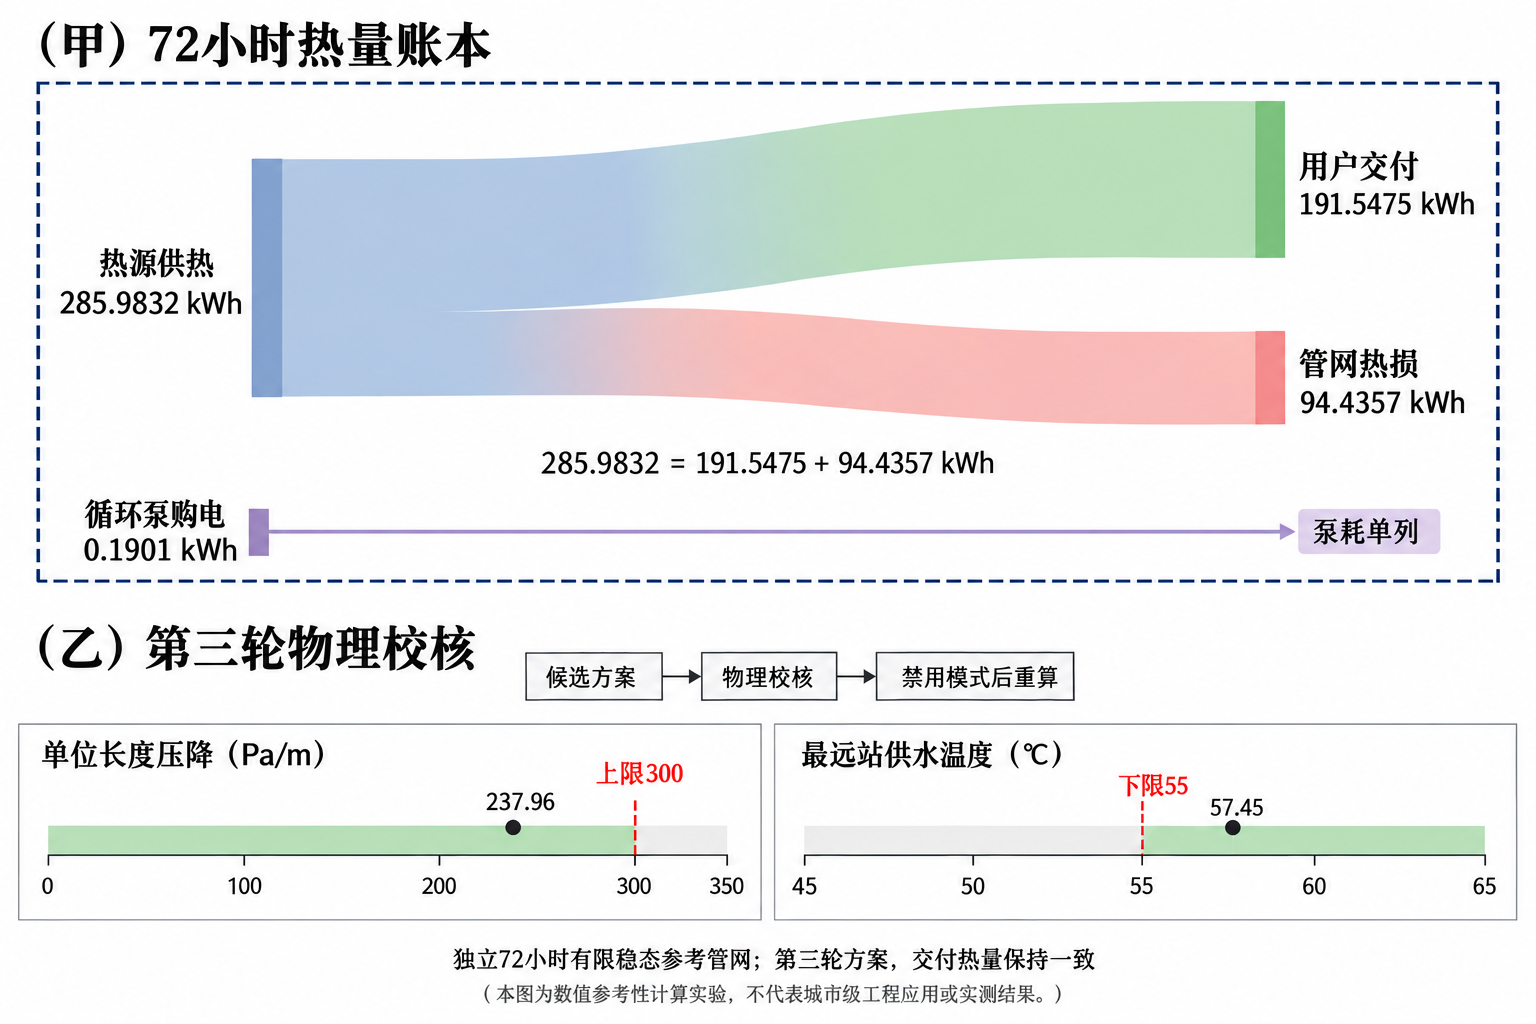
\includegraphics[width=0.96\linewidth]{results-a3/energy_balance_a3.png}
\caption[72小时参考管网的热量账本与物理校核]{72小时参考管网的热量账本与物理校核。循环泵购电单列；流带及点位示意分配关系与阈值比较，精确值以标注为准。仅在校核失败时禁用模式后重算；第三轮通过两项阈值后结束，前两轮与费用变化保留于本节表格。}
\label{fig:r8p-energy-a3}
\end{figure}

每轮时限60秒、目标gap0，均保留原求解状态、gap0与物理检查的分离记录。达标轮的历史结果属性因原浮点下界略大于可行值而保守记为缺证据，不升级为严格全局证明；物理可行审计仍通过。该有限稳态检查未覆盖冷启动、运输时滞、共泵水力平衡、RC脉冲舒适度、投资或动态故障认证。

\noindent\textbf{记录入口：}\path{docs/implementation_20261002_followup/parallel_stage_03/network/run_02/}，含\path{protocol.json}、\path{config.yaml}、\path{hourly.csv}、\path{comparison.json}、\path{manifest.json}与\path{failures.json}；\path{results/soft_off/history.json}和\path{results/soft_on/history.json}保留全部两轮拒绝及达标轮，不只展示最终通过点。

\subsection*{5.5\quad E08：四楼固定投资连续状态检查}
该组是武汉已登记合成参数数学场景，以相同规划方案冻结投资后复算四个独立建筑状态，并非四楼现场测温验证。服务年为北京时间2023年7月1日至2024年7月1日，共8784小时；声明冬季为2023年11月15日至2024年3月16日，共2928小时，均含起点、不含终点。

\begin{table}[H]
\centering
\caption{四楼两组连续窗口全部结果与运行层属性}
\begin{tabularx}{\linewidth}{@{}YrrL{0.22\linewidth}@{}}
\toprule
项目 & 服务年 & 声明冬季 & 解释\\\midrule
小时 & 8784 & 2928 & 单个连续窗口\\
交付热量/kWh & 958337.82 & 930728.48 & 四楼合计\\
交付冷量/kWh & 1327093.47 & 711.22 & 冷服务另核\\
现金运行费/元 & 285195.84 & 122974.20 & 仅对应本窗口\\
求解gap/\% & 0.1344 & 0.4755 & 请求容差0.5\%\\
求解时间/s & 133.07 & 48.21 & 总墙钟另留存\\
最大RC残差/$^\circ$C & $1.10\times10^{-13}$ & $6.75\times10^{-14}$ & 独立逐楼复算\\
舒适/初末违约 & 0/0 & 0/0 & 登记边界内\\
\bottomrule
\end{tabularx}
\end{table}

服务年现金总成本按纠正账本为586978.7050元，其中年化资本301782.8654元已包含一次；不能再次叠加资本。声明冬季122974.2004元只作同期运行费，不折成年费用、利润或回收期。两组运行请求时限分别1800/900秒，均在0.5\%登记容差内报告Optimal且状态检查通过，含固定投资标记、数值审计及新增投资零检查；仍不能说明投资计划联合最优。来源等级记录保留低等级设备参数，RC检查范围不替代热源、网络或真实建筑校准。

\noindent\textbf{记录入口：}原工程\path{outputs/competition_20261001/C4/optimized_annual_01/}与\path{outputs/competition_20261001/C4/optimized_season_03/}的\path{run_record.json}、\path{summary.json}、\path{independent_rc_audit.json}、\path{c6_building_audit.json}、\path{corrected_cost.json}及逐时轨迹。既有R8L源包\path{evidence/C4/ARCHIVE_INDEX.json}登记原路径、原SHA与无损gzip副本；本轮核对压缩身份及解压原身份，不修改其历史来源审核状态。

\subsection*{5.6\quad E09：三城27条固定策略的全部六方法}
该组为已见三城的开发确认。每城2880小时、九策略、同八个真实代表日；六方法均先于真实策略电费/能耗完成校准。三城27条完整轨迹共77760小时，不声称减少仿真量。九策略编号0--8依次为零预热、全谷段1/3~$^\circ$C、05时末端1/3~$^\circ$C、13时末端1/3~$^\circ$C、双末端1/3~$^\circ$C；跨日状态继承、自然漂移上限27~$^\circ$C、最后一小时恢复20~$^\circ$C并计冷热能量。

预算均以各城同一完整季零预热电量为基线，倍率1、1.02、1.05、1.10；固定碳因子使能量/碳帽冗余。按估计费用在估计帽内选策略，费用并列容差$10^{-8}$元，再按最小策略编号；实际帽与服务另核，无估计可行策略不回退。遗憾只对实际可行选择计算，超帽/无选择留空；oracle只在相同九策略库内，不是全局调度最优。

\begin{table}[H]
\centering
\caption{六方法完整27策略估计与12次选择分母；误差列为\%}
\begin{tabularx}{\linewidth}{@{}Yrrrrr@{}}
\toprule
方法简名 & \shortstack{电费\\MAPE} & \shortstack{能量\\MAPE} & \shortstack{最大能量\\APE} & 合格/12 & 超帽/无选\\\midrule
频数 & 0.556911 & 0.267761 & 0.718644 & 9 & 2/1\\
软能量 & 0.448316 & 0.044228 & 0.291601 & 11 & 0/1\\
硬$W_1$ & 0.140535 & 0.057807 & 0.315063 & 12 & 0/0\\
硬最小$L_1$ & 0.460634 & 0.043351 & 0.289511 & 12 & 0/0\\
价/时窗配对$L_1$ & 0.485844 & 0.050416 & 0.289022 & 12 & 0/0\\
硬$W_1$加候选$L_1$上限 & 0.329306 & 0.045621 & 0.290410 & 12 & 0/0\\
\bottomrule
\end{tabularx}
\end{table}

\begin{table}[H]
\centering
\caption{电费MAPE的逐城分解，单位为\%}
\begin{tabularx}{\linewidth}{@{}Yrrr@{}}
\toprule
方法 & 乌鲁木齐 & 固原 & 武汉\\\midrule
频数 & 0.772160 & 0.094224 & 0.804347\\
软能量 & 0.698834 & 0.288920 & 0.357193\\
硬$W_1$ & 0.018529 & 0.341666 & 0.061409\\
硬最小$L_1$ & 0.696076 & 0.300437 & 0.385390\\
价/时窗配对$L_1$ & 0.523837 & 0.300437 & 0.633258\\
硬$W_1$加候选$L_1$上限 & 0.075426 & 0.300437 & 0.612056\\
\bottomrule
\end{tabularx}
\end{table}

\begin{table}[H]
\centering
\caption{全部城市与预算的选择；四种硬方法逐例同选，故合并显示}
\begin{tabularx}{\linewidth}{@{}Yrrrr@{}}
\toprule
城市/帽倍率 & 频数 & 软能量 & 四种硬方法 & 库内oracle\\\midrule
乌鲁木齐/1.00 & 无选 & 无选 & 0 & 0\\
乌鲁木齐/1.02 & 8 & 8 & 8 & 8\\
乌鲁木齐/1.05 & 8 & 8 & 8 & 8\\
乌鲁木齐/1.10 & 8 & 8 & 8 & 8\\
固原/1.00 & 3超帽 & 0 & 0 & 0\\
固原/1.02 & 8 & 8 & 8 & 8\\
固原/1.05 & 8 & 8 & 8 & 8\\
固原/1.10 & 8 & 8 & 8 & 8\\
武汉/1.00 & 3超帽 & 0 & 0 & 0\\
武汉/1.02 & 4 & 4 & 4 & 4\\
武汉/1.05 & 8 & 8 & 8 & 8\\
武汉/1.10 & 8 & 8 & 8 & 8\\
\bottomrule
\end{tabularx}
\end{table}

频数的两次超帽分别为12.5160、12.6716~kWh，原遗憾留空；不能把九次有效遗憾为0改说成12次全部成功。四种硬法均12次实际合格且选到库内oracle，遗憾均0，故没有新候选优于硬$W_1$选策的证据。冻结规则按合格数、遗憾、最大能量APE等排序，仍登记价/时窗配对$L_1$；其最大能量APE比最小$L_1$仅低0.000489个百分点，电费MAPE却约为硬$W_1$的3.46倍。固原硬$W_1$电费MAPE还高于频数，逐城结果不能被总平均掩盖。代理热量守恒不等于策略电量/电费精确，价格矩和05/13时窗约束共同改变，不能据联合候选单独证明价格矩因果贡献。

独立42225项记录检查及全部27轨迹RC/服务/初末/容量/互斥检查通过；首次审计因两处约$9.09\times10^{-13}$元的并列翻位失败，原记录保留，补充精度审计未改权重、协议或阈值。运行29.135秒、共同准备0.648秒分别记录，全真值计算计入成本；不把不同方法的依赖成本或仿真成本省略后声称提速。

\noindent\textbf{记录入口：}\path{docs/implementation_20261002_followup/parallel_stage_03/algorithm/}，含\path{confirmation_run_01/protocol.json}、\path{manifest.json}、\path{truth.json}、\path{selections.json}、\path{predictions.json}、\path{failures.json}、完整轨迹与逐日表；\path{analysis_01/method_summary.csv}、\path{budget_selections.csv}及\path{policy_predictions.csv}保存完整分母，\path{claims_reviewed.txt}、\path{interpretation.json}和\path{verification_02/audit.json}限定结论。原三城天气已用于开发，模型为共同公开原型及方法学电价；无新留出泛化、实际投资改善或在线预测主张。

\subsection*{5.7\quad 身份、复算范围与交付说明}
本轮R8P对既有证据索引和新增引用文件计算SHA-256，并从保存的JSON/CSV重新汇总六楼中位数、采用分母、热容四格差值和27策略误差，核对正文及附录的舍入数值；不重新运行求解器、不累计历史测试，也不将此前通过记录改成本轮新实验。完整小时调度留在各原证据目录，附录展示所有实验单元与拒绝/超帽/无选分母，不打印数万小时流水。

正文保留\path{minor:supplement}标题锚点，表\ref{tab:r8p-comparisons}仅列E01/E03；原\path{tab:minor-evidence}移至本附录总表，仍含管网反馈和四楼连续状态，因而主文工程反馈、创新及评分页的原交叉引用没有变成另一组实验。历史结果的原始来源、模型版本、投资范围、求解容差和适用限制随记录保留。
